\documentclass{beamer}

% Theme choices
\usetheme{Madrid}
\usecolortheme{dolphin}
\usefonttheme{professionalfonts}

\usepackage{svg}
\usepackage{minted}
\usepackage{xcolor}


% Define colors for code highlighting
\definecolor{codebg}{rgb}{0.95,0.95,0.95}

% Minted settings
% Set the style for syntax highlighting
\usemintedstyle{friendly}

% ----------------------------------------------------------------------------------------------------------------
% --- document ---------------------------------------------------------------------------------------------------
% ----------------------------------------------------------------------------------------------------------------

% Title page details
\title[Advent of Code 2022 Day 14]{Advent of Code 2022 Day 14}
\author{Simon Roller}
\institute{University of Tübingen}
\date{\today} % todo-----------------------------------------------------------------------------------------------

\begin{document}

% Title page
\begin{frame}
    \titlepage
\end{frame}

\section{Motivation}

\begin{frame}{Motivation}
How much sand is needed to fill the cave and its surroundings?
    \begin{figure}[H]
        \centering
        \includesvg[width=0.5\textwidth]{Images/AoC22_14_00.svg}
    \end{figure}
\end{frame}

\section{Problem Example}

%\begin{frame}{Problem Example}
%only offline
%\end{frame}

\begin{frame}{Problem Example}
    \begin{figure}[H]
        \centering
        \includesvg[width=0.5\textwidth]{Images/AoC22_14_01.svg}
    \end{figure}
\end{frame}
\begin{frame}
    \begin{figure}[H]
        \centering
        \includesvg[width=0.5\textwidth]{Images/AoC22_14_02.svg}
    \end{figure}
\end{frame}
\begin{frame}
    \begin{figure}[H]
        \centering
        \includesvg[width=0.5\textwidth]{Images/AoC22_14_03.svg}
    \end{figure}
\end{frame}
\begin{frame}
    \begin{figure}[H]
        \centering
        \includesvg[width=0.5\textwidth]{Images/AoC22_14_04.svg}
    \end{figure}
\end{frame}
\begin{frame}
    \begin{figure}[H]
        \centering
        \includesvg[width=0.5\textwidth]{Images/AoC22_14_05.svg}
    \end{figure}
\end{frame}
\begin{frame}
    \begin{figure}[H]
        \centering
        \includesvg[width=0.5\textwidth]{Images/AoC22_14_06.svg}
    \end{figure}
\end{frame}
\begin{frame}
    \begin{figure}[H]
        \centering
        \includesvg[width=0.5\textwidth]{Images/AoC22_14_07.svg}
    \end{figure}
\end{frame}
\begin{frame}
    \begin{figure}[H]
        \centering
        \includesvg[width=0.5\textwidth]{Images/AoC22_14_08.svg}
    \end{figure}
\end{frame}
\begin{frame}
    \begin{figure}[H]
        \centering
        \includesvg[width=0.5\textwidth]{Images/AoC22_14_09.svg}
    \end{figure}
\end{frame}
\begin{frame}
    \begin{figure}[H]
        \centering
        \includesvg[width=0.5\textwidth]{Images/AoC22_14_10.svg}
    \end{figure}
\end{frame}
\begin{frame}
    \begin{figure}[H]
        \centering
        \includesvg[width=0.5\textwidth]{Images/AoC22_14_11.svg}
    \end{figure}
\end{frame}
\begin{frame}
    \begin{figure}[H]
        \centering
        \includesvg[width=0.5\textwidth]{Images/AoC22_14_12.svg}
    \end{figure}
\end{frame}
\begin{frame}
    \begin{figure}[H]
        \centering
        \includesvg[width=0.5\textwidth]{Images/AoC22_14_13.svg}
    \end{figure}
\end{frame}
\begin{frame}
    \begin{figure}[H]
        \centering
        \includesvg[width=0.5\textwidth]{Images/AoC22_14_14.svg}
    \end{figure}
\end{frame}
\begin{frame}
    \begin{figure}[H]
        \centering
        \includesvg[width=0.5\textwidth]{Images/AoC22_14_15.svg}
    \end{figure}
\end{frame}
\begin{frame}
    \begin{figure}[H]
        \centering
        \includesvg[width=0.5\textwidth]{Images/AoC22_14_16.svg}
    \end{figure}
\end{frame}
\begin{frame}
    \begin{figure}[H]
        \centering
        \includesvg[width=0.5\textwidth]{Images/AoC22_14_17.svg}
    \end{figure}
\end{frame}
\begin{frame}
    \begin{figure}[H]
        \centering
        \includesvg[width=0.5\textwidth]{Images/AoC22_14_18.svg}
    \end{figure}
\end{frame}
\begin{frame}
    \begin{figure}[H]
        \centering
        \includesvg[width=0.5\textwidth]{Images/AoC22_14_19.svg}
    \end{figure}
\end{frame}
\begin{frame}
    \begin{figure}[H]
        \centering
        \includesvg[width=0.5\textwidth]{Images/AoC22_14_20.svg}
    \end{figure}
\end{frame}
\begin{frame}
    \begin{figure}[H]
        \centering
        \includesvg[width=0.5\textwidth]{Images/AoC22_14_21.svg}
    \end{figure}
\end{frame}
\begin{frame}
    \begin{figure}[H]
        \centering
        \includesvg[width=0.5\textwidth]{Images/AoC22_14_22.svg}
    \end{figure}
\end{frame}
\begin{frame}
    \begin{figure}[H]
        \centering
        \includesvg[width=0.5\textwidth]{Images/AoC22_14_23.svg}
    \end{figure}
\end{frame}
\begin{frame}
    \begin{figure}[H]
        \centering
        \includesvg[width=0.5\textwidth]{Images/AoC22_14_24.svg}
    \end{figure}
\end{frame}
\begin{frame}
    \begin{figure}[H]
        \centering
        \includesvg[width=0.5\textwidth]{Images/AoC22_14_25.svg}
    \end{figure}
\end{frame}
\begin{frame}
    \begin{figure}[H]
        \centering
        \includesvg[width=0.5\textwidth]{Images/AoC22_14_26.svg}
    \end{figure}
\end{frame}
\begin{frame}
    \begin{figure}[H]
        \centering
        \includesvg[width=0.5\textwidth]{Images/AoC22_14_27.svg}
    \end{figure}
\end{frame}
\begin{frame}
    \begin{figure}[H]
        \centering
        \includesvg[width=0.5\textwidth]{Images/AoC22_14_28.svg}
    \end{figure}
\end{frame}
\begin{frame}
    \begin{figure}[H]
        \centering
        \includesvg[width=0.5\textwidth]{Images/AoC22_14_29.svg}
    \end{figure}
\end{frame}



\section{Programming Language}

\begin{frame}{Programming Language}
    \begin{minipage}[c]{0.4\textwidth}
        \begin{itemize}
            \item ease of use
        \end{itemize}
    \end{minipage}%
    \begin{minipage}[c]{0.6\textwidth}
        \begin{figure}[H]
            \centering
            
\includegraphics[width=0.5\textwidth]{Images/python_logo.png}
        \end{figure}
    \end{minipage}
\end{frame}

\begin{frame}{Programming Language}
    \begin{minipage}[c]{0.4\textwidth}
        \begin{itemize}
            \item ease of use
            \item no runtime or memory constraints
        \end{itemize}
    \end{minipage}%
    \begin{minipage}[c]{0.6\textwidth}
        \begin{figure}[H]
            \centering
            
\includegraphics[width=0.5\textwidth]{Images/python_logo.png}
        \end{figure}
    \end{minipage}
\end{frame}

\begin{frame}{Programming Language}
    \begin{minipage}[c]{0.4\textwidth}
        \begin{itemize}
            \item ease of use
            \item no runtime or memory constraints
            \item me being proficient in the language
        \end{itemize}
    \end{minipage}%
    \begin{minipage}[c]{0.6\textwidth}
        \begin{figure}[H]
            \centering
            
\includegraphics[width=0.5\textwidth]{Images/python_logo.png}
        \end{figure}
    \end{minipage}
\end{frame}

\section{Input Details}

\begin{frame}[fragile]{Input Details}
    \begin{minted}[bgcolor=codebg, linenos, fontsize=\footnotesize]{python}
498,4 -> 498,6 -> 496,6
503,4 -> 502,4 -> 502,9 -> 494,9
    \end{minted}
\end{frame}
\begin{frame}[fragile]{Input Details}
    \begin{minted}[bgcolor=codebg, linenos, fontsize=\footnotesize]{python}
498,4 -> 498,6 -> 496,6
503,4 -> 502,4 -> 502,9 -> 494,9
    \end{minted}
    \begin{minipage}[c]{0.4\textwidth}
        \begin{figure}[H]
            \centering
            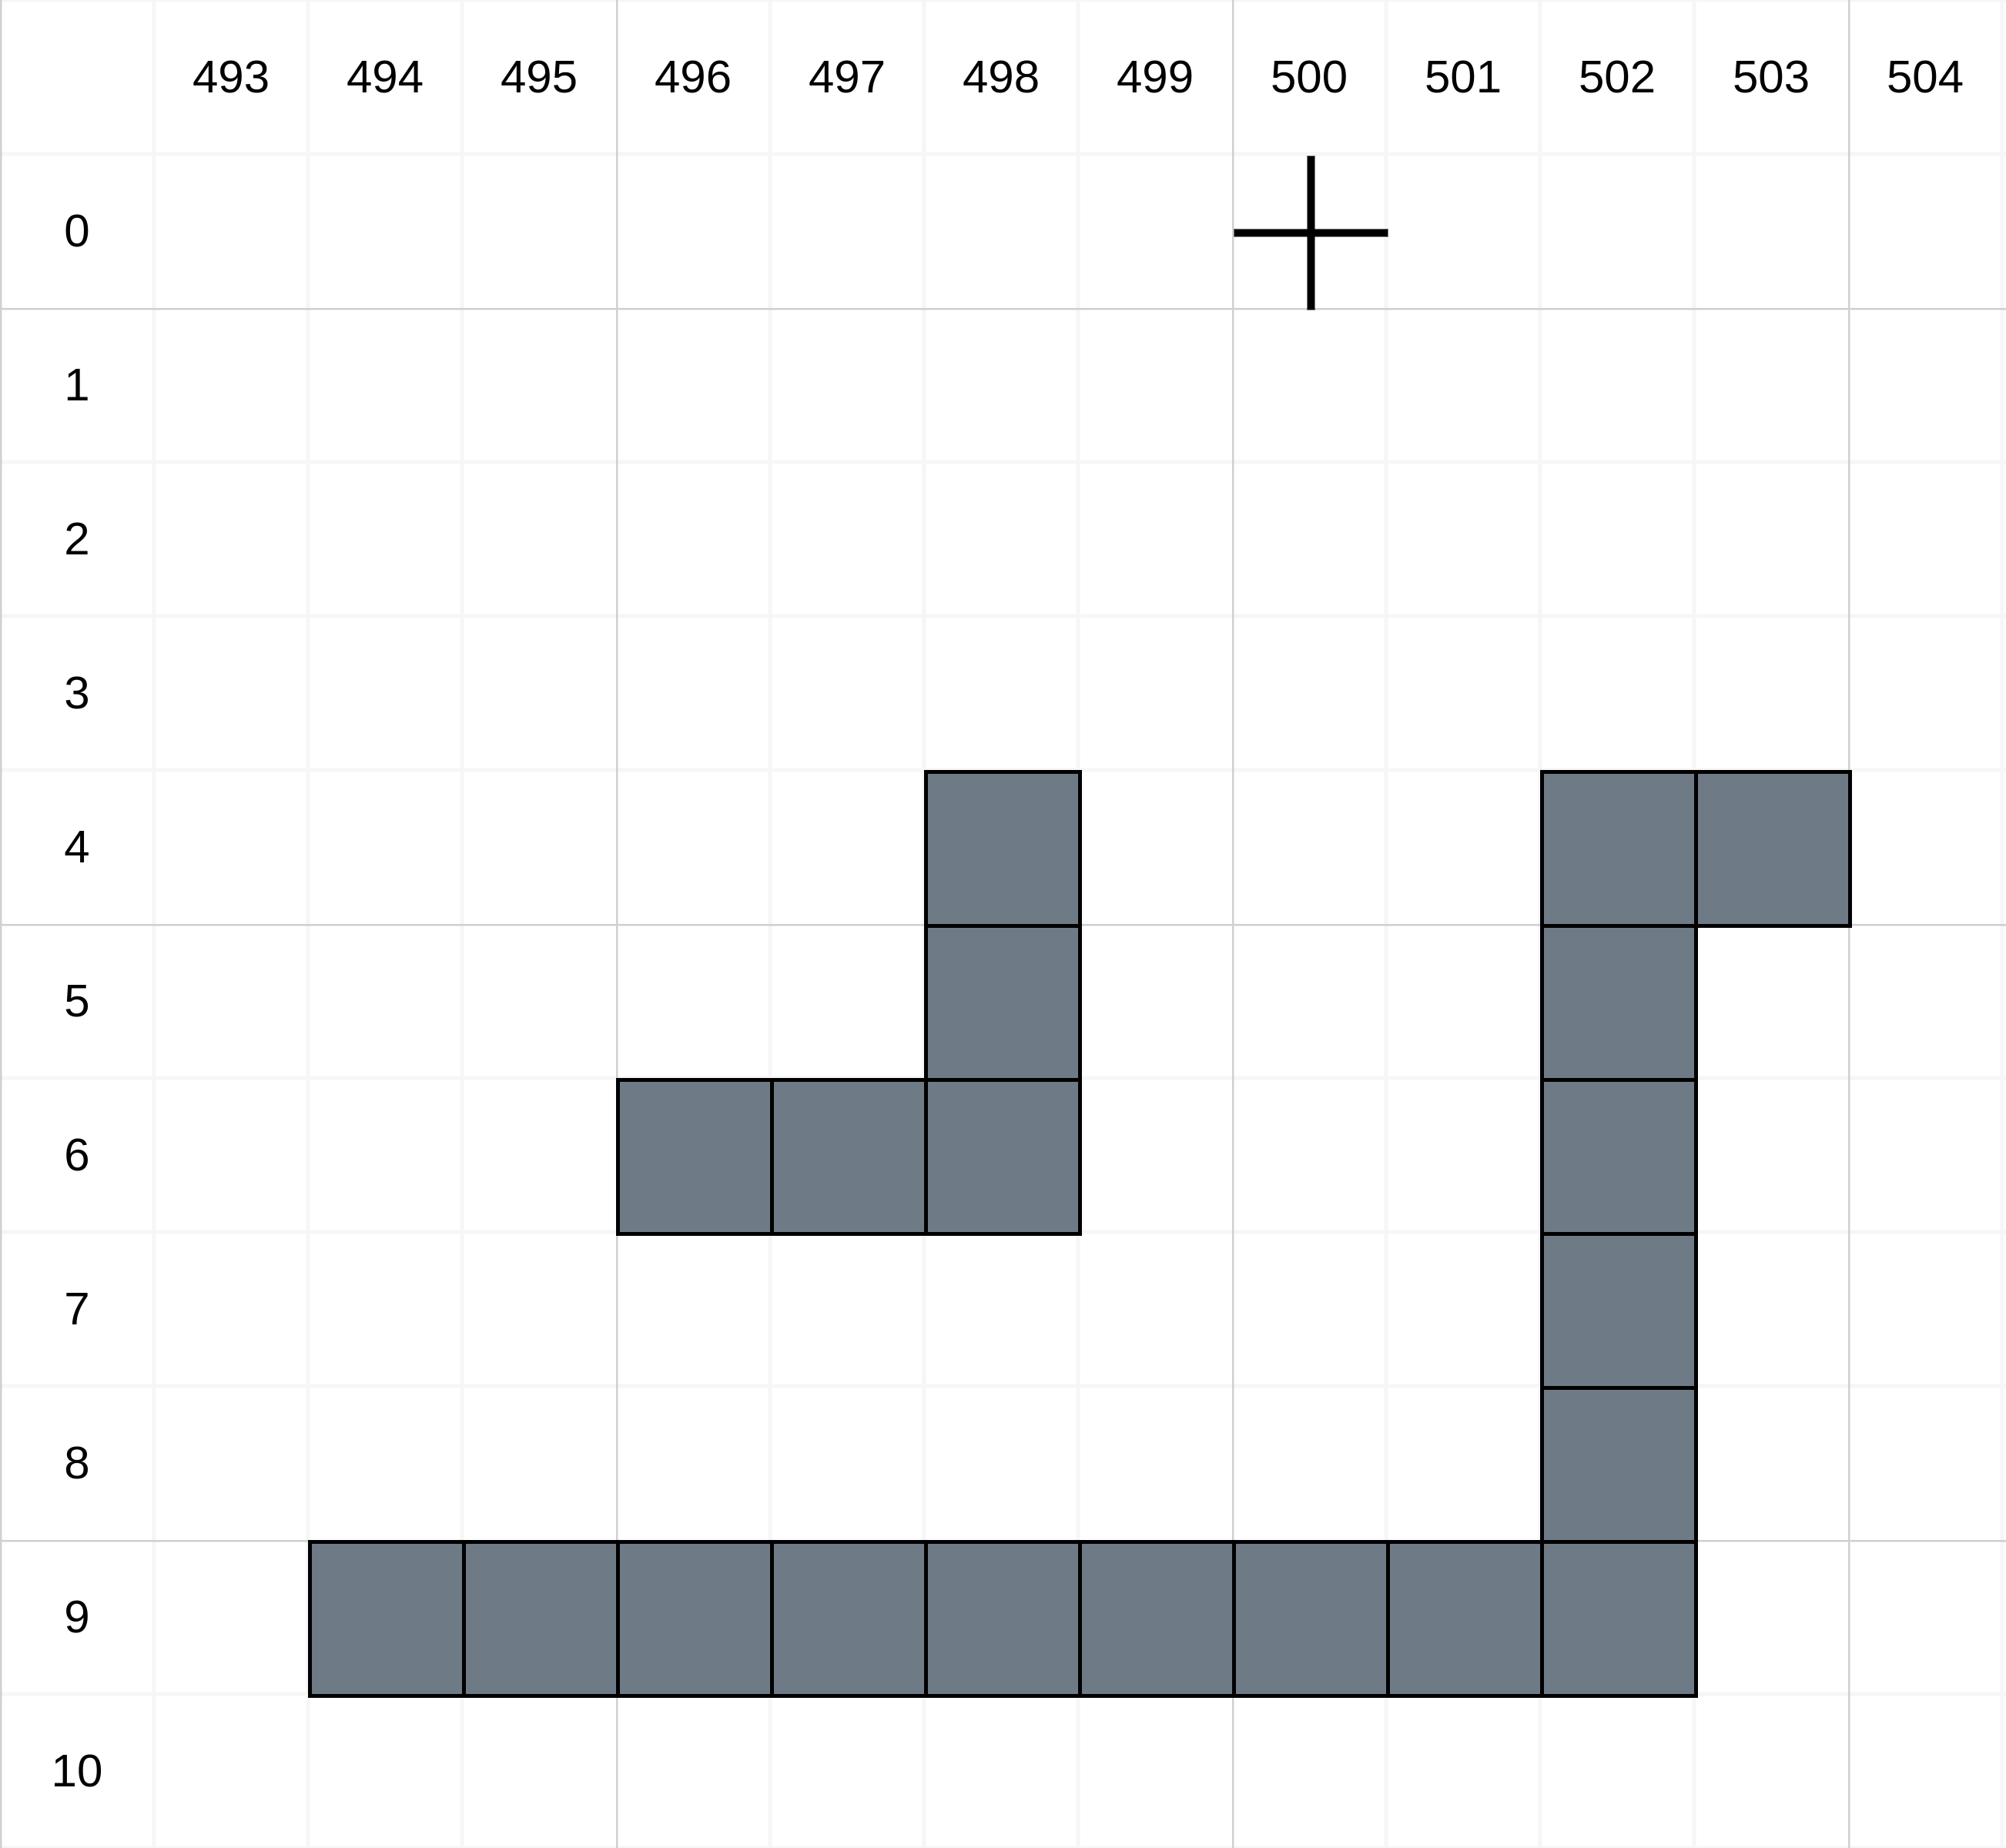
\includegraphics[width=0.8\textwidth]{Images/AoC22_14_00_grid.png}
        \end{figure}
    \end{minipage}%
    \begin{minipage}[c]{0.6\textwidth}
        \begin{figure}[H]
            \centering
            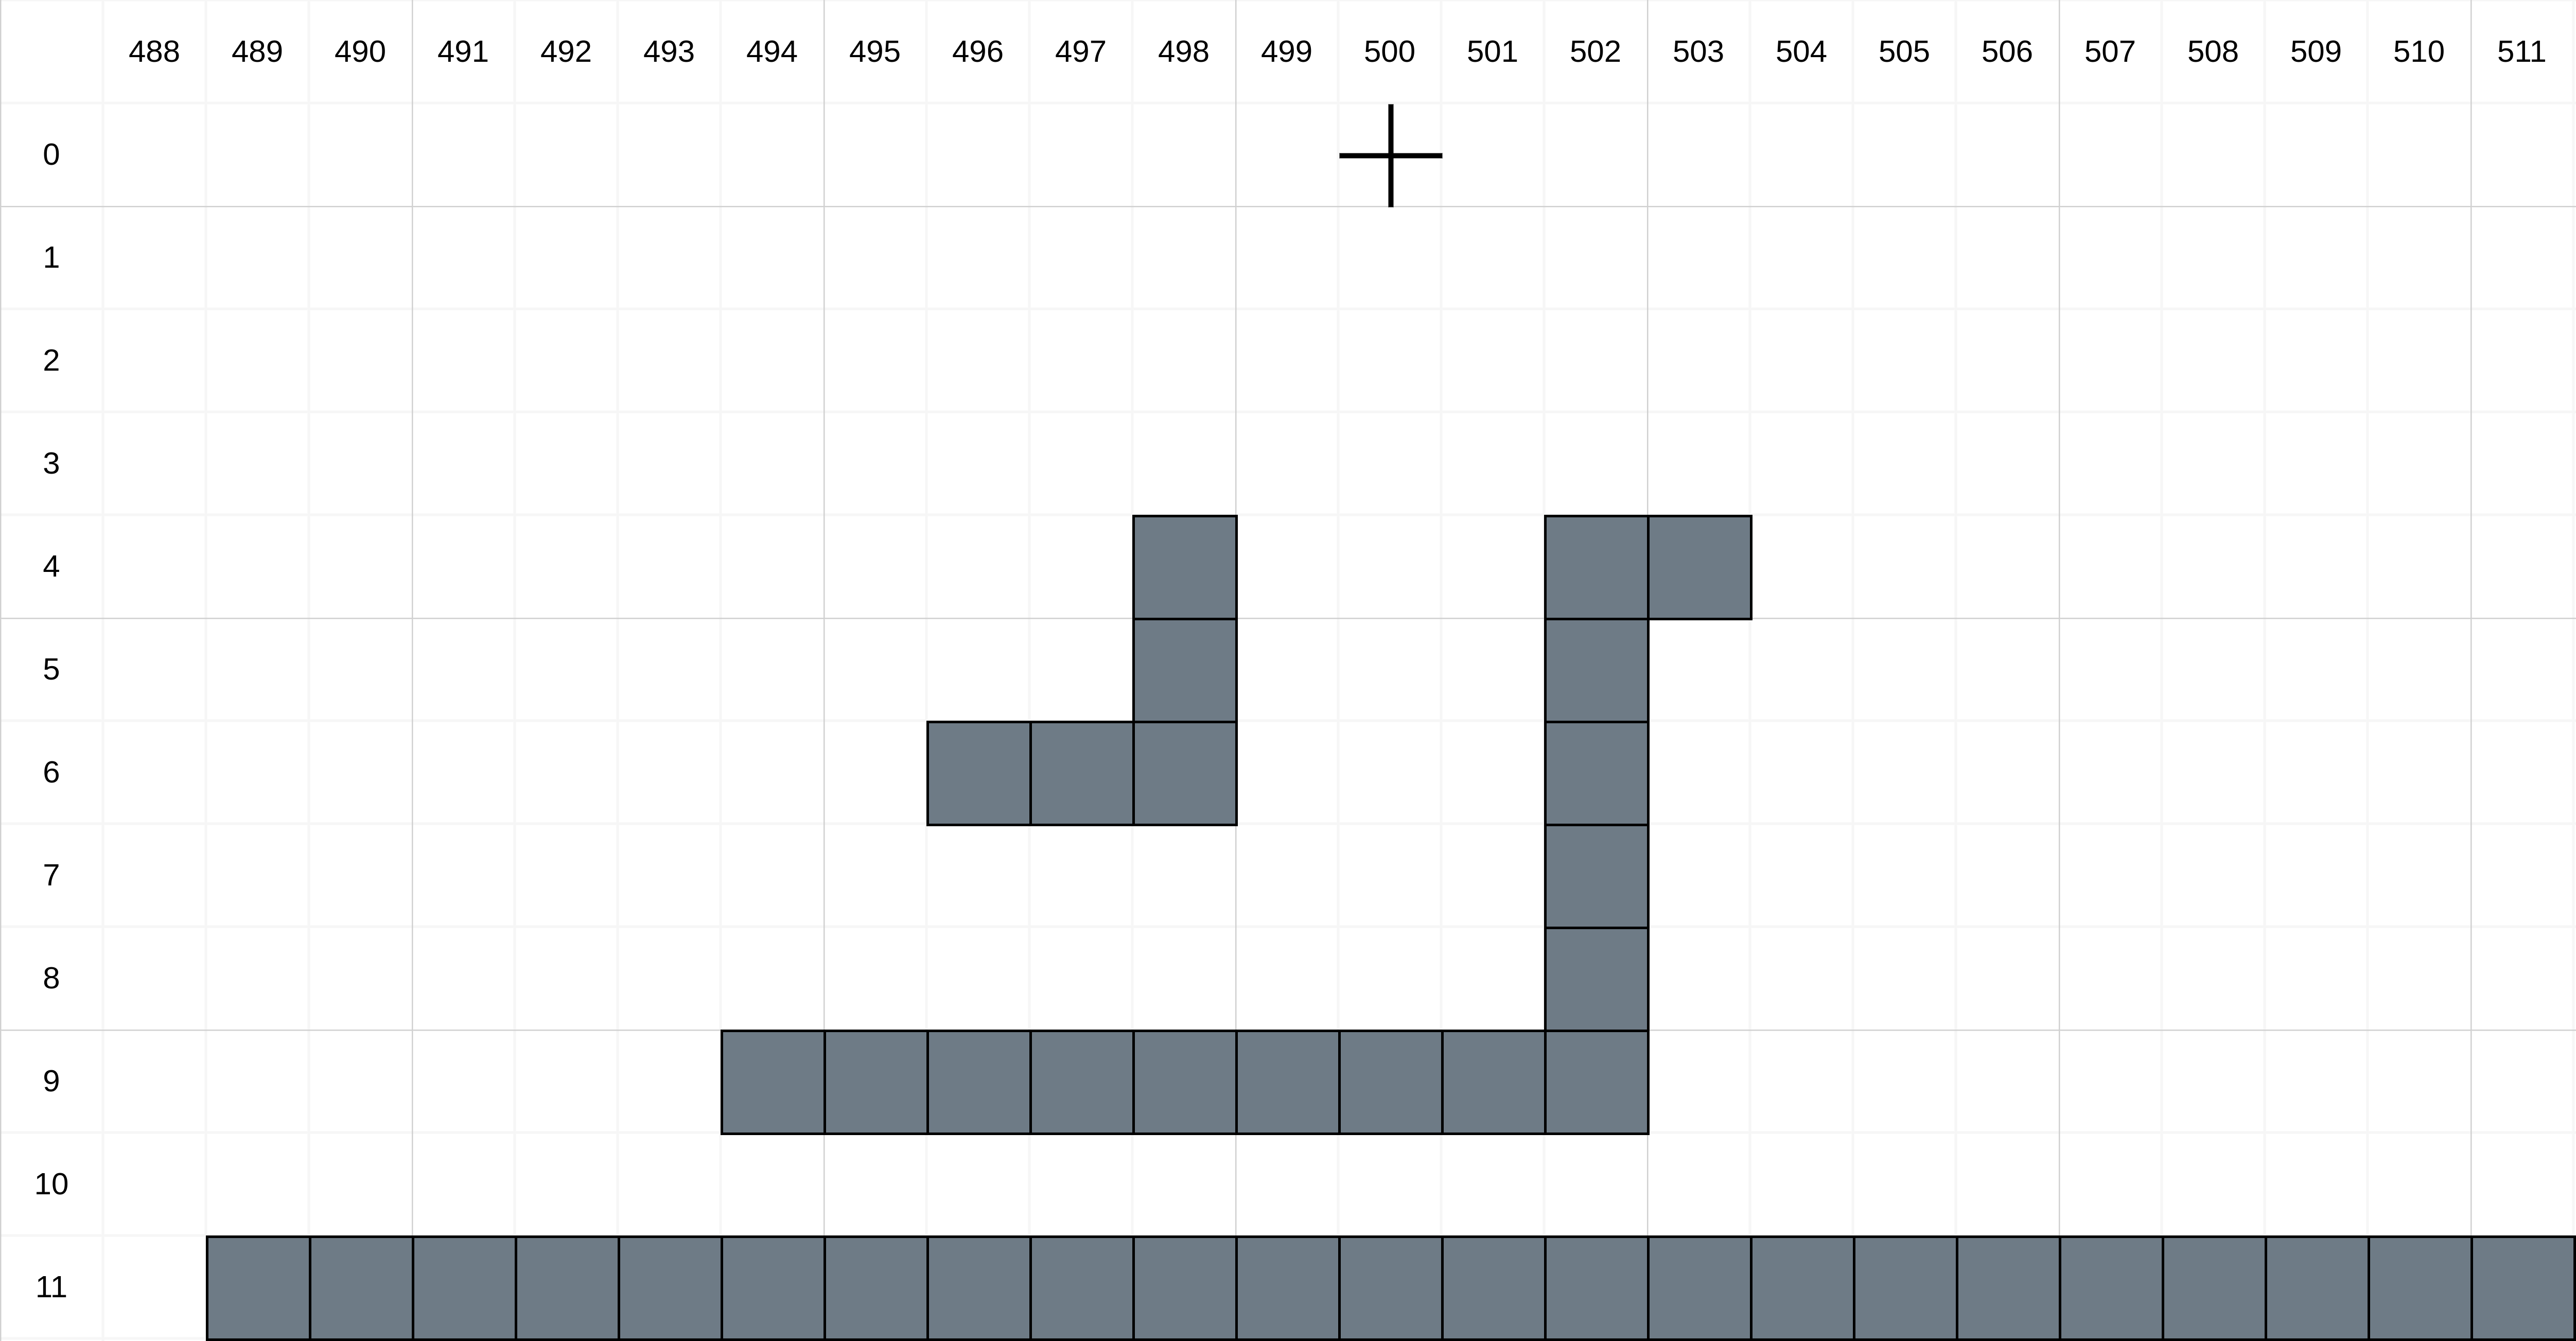
\includegraphics[width=0.8\textwidth]{Images/AoC22_14_Part_2_0_grid.png}
        \end{figure}
    \end{minipage}
\end{frame}

\section{Output Details}

\begin{frame}{Output Details}
    \begin{itemize}
        \item Part 1: 24
        \item Part 2: 93
    \end{itemize}
\end{frame}
\section{Solution Approach}

\begin{frame}{Solution Approach}
    \begin{figure}[H]
        \centering
        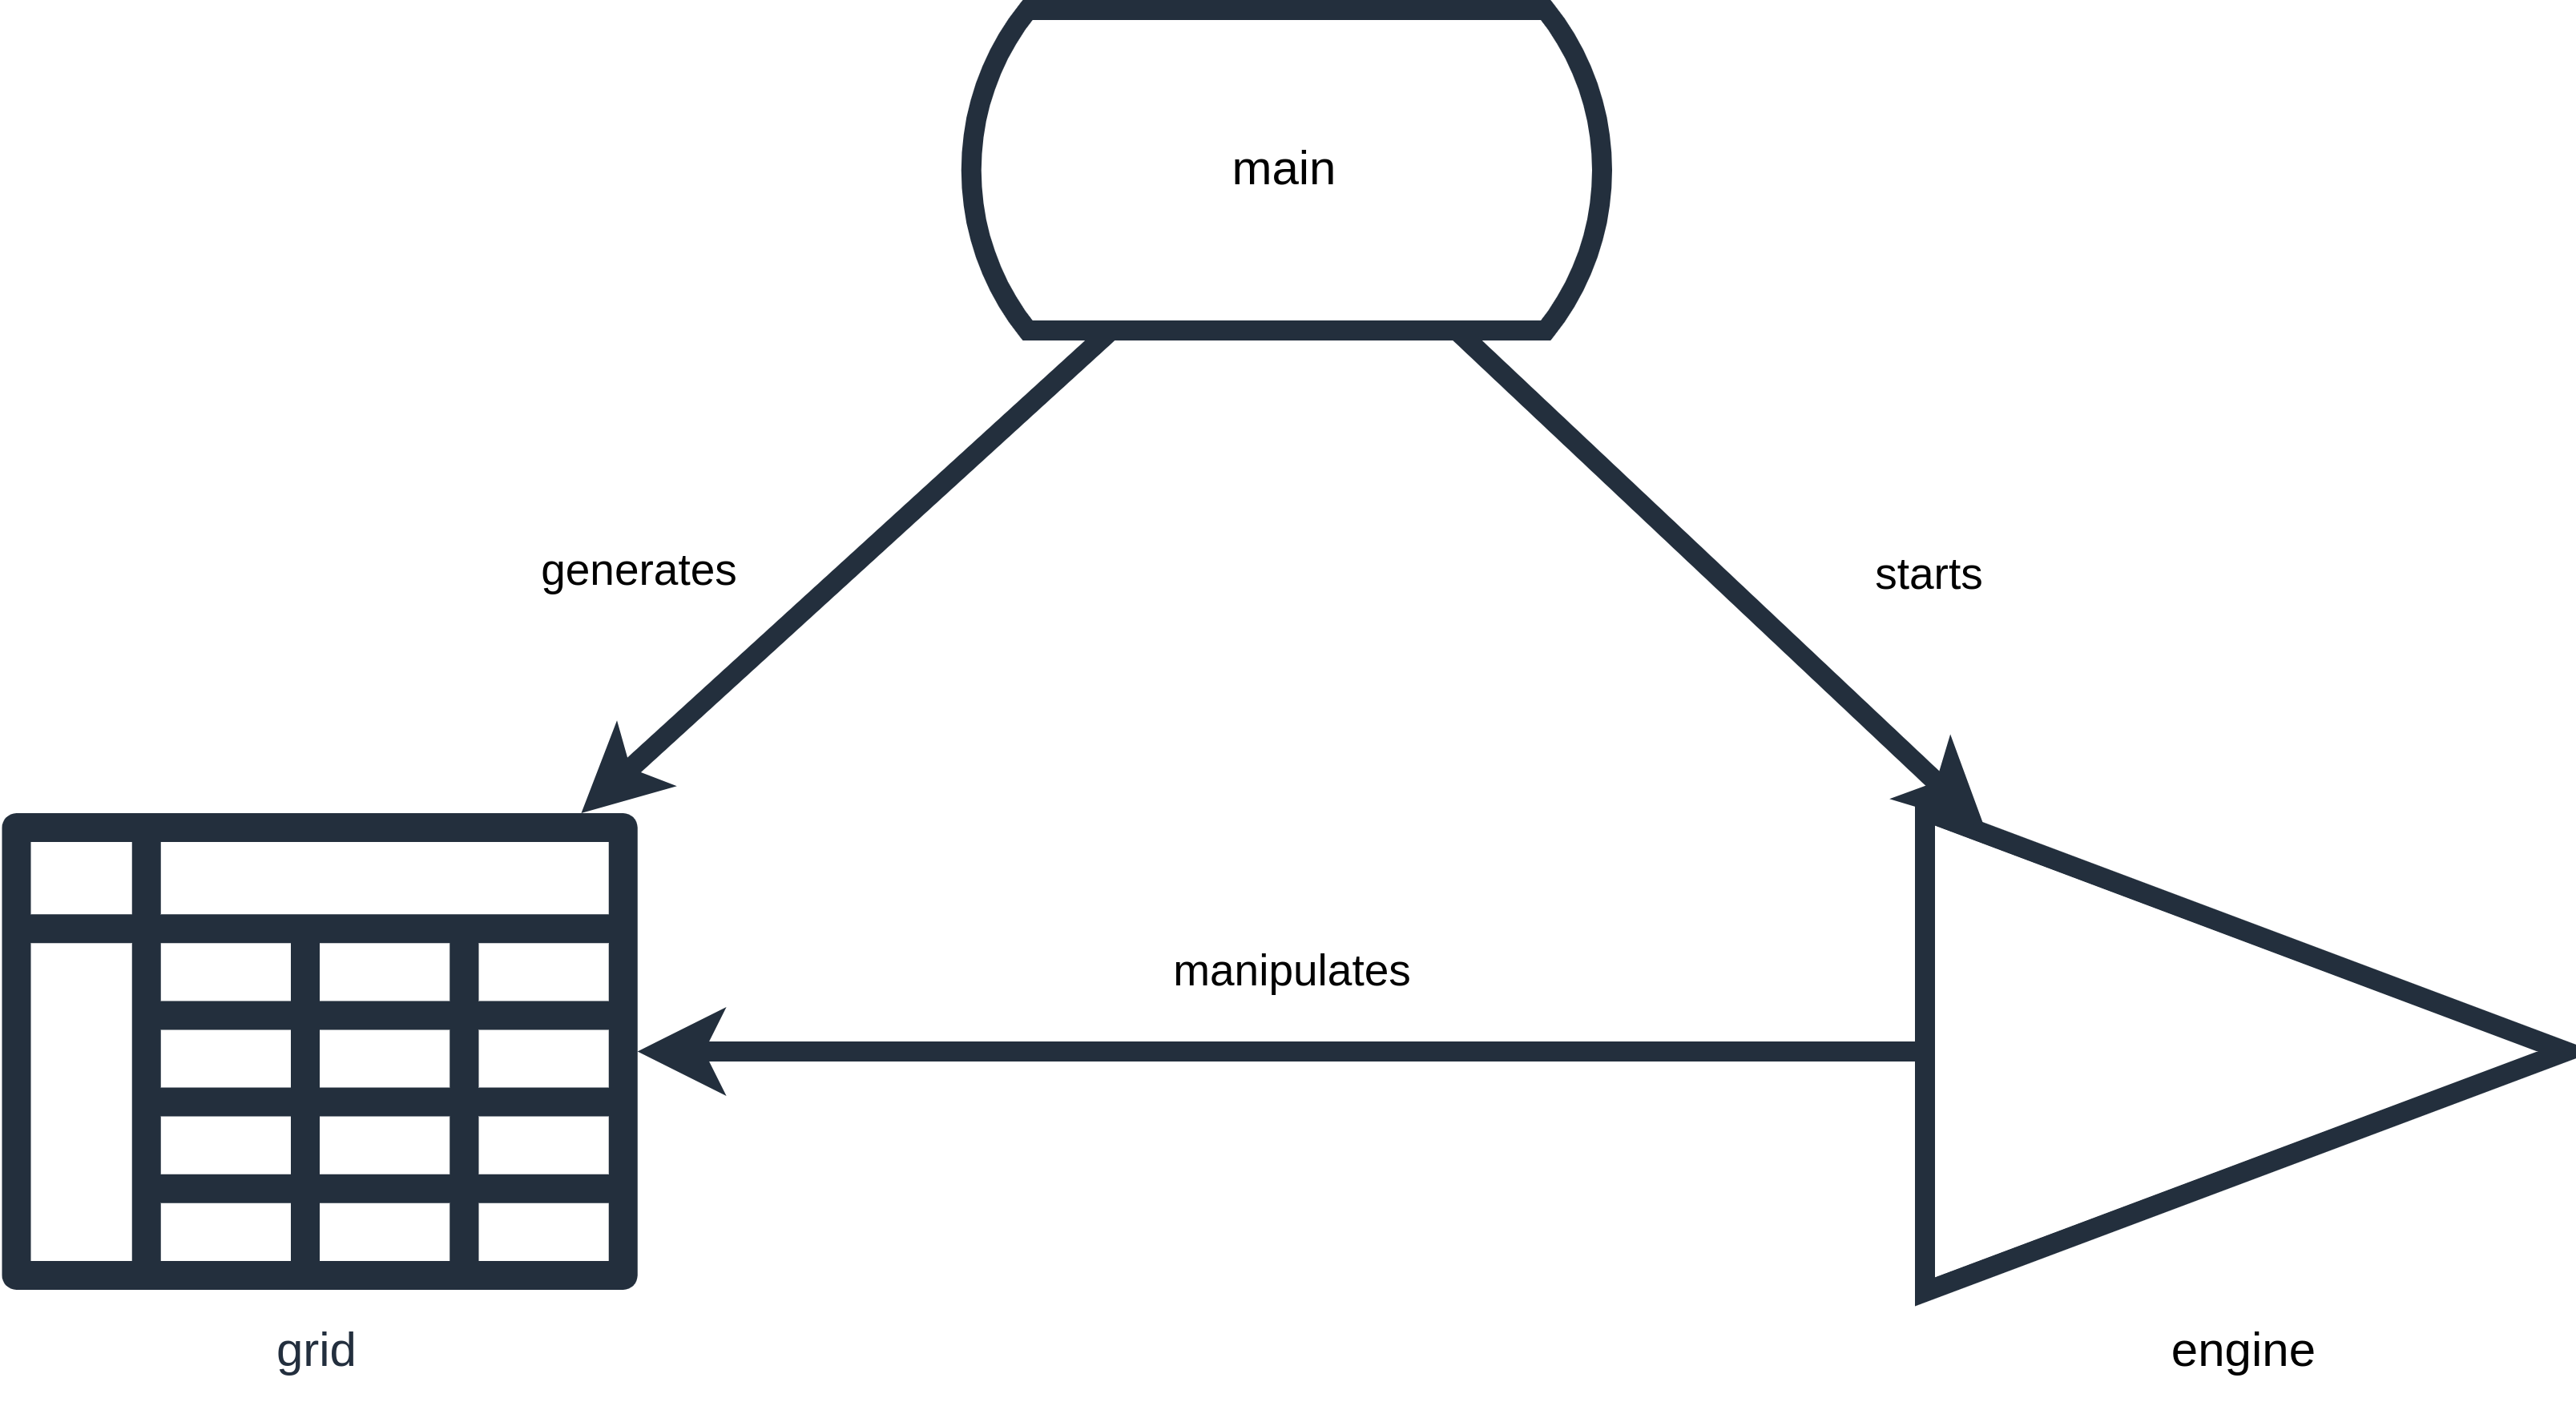
\includegraphics[width=0.8\textwidth]{Images/AoC22_14_high_level.png}
    \end{figure}
\end{frame}

% optionally also show grid generation
\section{Code Example}

\begin{frame}[fragile]{Code Example}
    \begin{minted}[bgcolor=codebg, linenos, fontsize=\scriptsize]{python}
num = 0
while True:
    sand = (500, 0)
    while True:
        if self.grid.is_air_at(Coordinate((sand[0], sand[1] + 1))):
            sand = (sand[0], sand[1] + 1)
        elif self.grid.is_air_at(Coordinate((sand[0] - 1, sand[1] + 1))):
            sand = (sand[0] - 1, sand[1] + 1)
        elif self.grid.is_air_at(Coordinate((sand[0] + 1, sand[1] + 1))):
            sand = (sand[0] + 1, sand[1] + 1)
        else:
            self.grid.add(Object((Material.solid_sand, Coordinate(sand))))
            break
        if sand[1] >= self.grid.get_last_row() + 1:
            if not part2:
                return num
            self.grid.add(Object((Material.solid_sand, Coordinate(sand))))
            break
    num += 1
    if sand == (500, 0):
        return num
    \end{minted}
\end{frame}

\section{Live Demo}

\begin{frame}{Live Demo}
\end{frame}

\section{Key Takeaways \& Outlook}

\begin{frame}{Key Takeaways \& Outlook}
    \begin{itemize}
        \item rock structure is created using the input coordinates
    \end{itemize}
\end{frame}

\begin{frame}{Key Takeaways \& Outlook}
    \begin{itemize}
        \item rock structure is created using the input coordinates
        \item dynamically calculate the number of sand
    \end{itemize}
\end{frame}

\begin{frame}{Key Takeaways \& Outlook}
    \begin{itemize}
        \item rock structure is created using the input coordinates
        \item dynamically calculate the number of sand
        \item adjust grid to be optimized for memory or computational performance
    \end{itemize}
\end{frame}

\begin{frame}{Key Takeaways \& Outlook}
    \begin{itemize}
        \item rock structure is created using the input coordinates
        \item dynamically calculate the number of sand
        \item adjust grid to be optimized for memory or computational performance
        \item render falling sand
    \end{itemize}
\end{frame}

\begin{frame}{Reference}
    \begin{thebibliography}{99}
        \bibitem{aoc} Advent of Code. \textit{Advent of Code 2022}. \url{https://adventofcode.com/2022/day/14}
    \end{thebibliography}
\end{frame}

\end{document}
